\section{Evaluation}

% - Executed within Linux Namespace Containers with CORE
% - Compare with Serval, IBR-DTN, Forban
% - Different Payloads:
%     - 64 KiB, compressed image
%     - 1 MiB, small image / short audio recording
%     - 5 MiB, smartphone image / audio recording
%     - 25 MiB, longer audio recording / short video
%     - 50 MiB, HD video
%     - 100 MiB, 4k smartphone video
% - Nodes are connected pairwise with a chain topology
%     - Three different lengths: 2 nodes, 32 nodes, 64 nodes
%     - Bandwith limited to 54 MBit/s, IEEE 802.11g network
% - Results: DTN7 and IBR-DTN are way faster for small files
%     - Time converges for bigger files, because of 54 MBit/s

\begin{frame}
  \frametitle{Evaluation}

  \begin{itemize}
  \item Up to 64 nodes emulated in the \acf{CORE}
  \item Nodes are connected pairwise in a chain topology
  \item Simulated IEEE 802.11g network, 54 MBit/s
  \end{itemize}

  \begin{figure}
    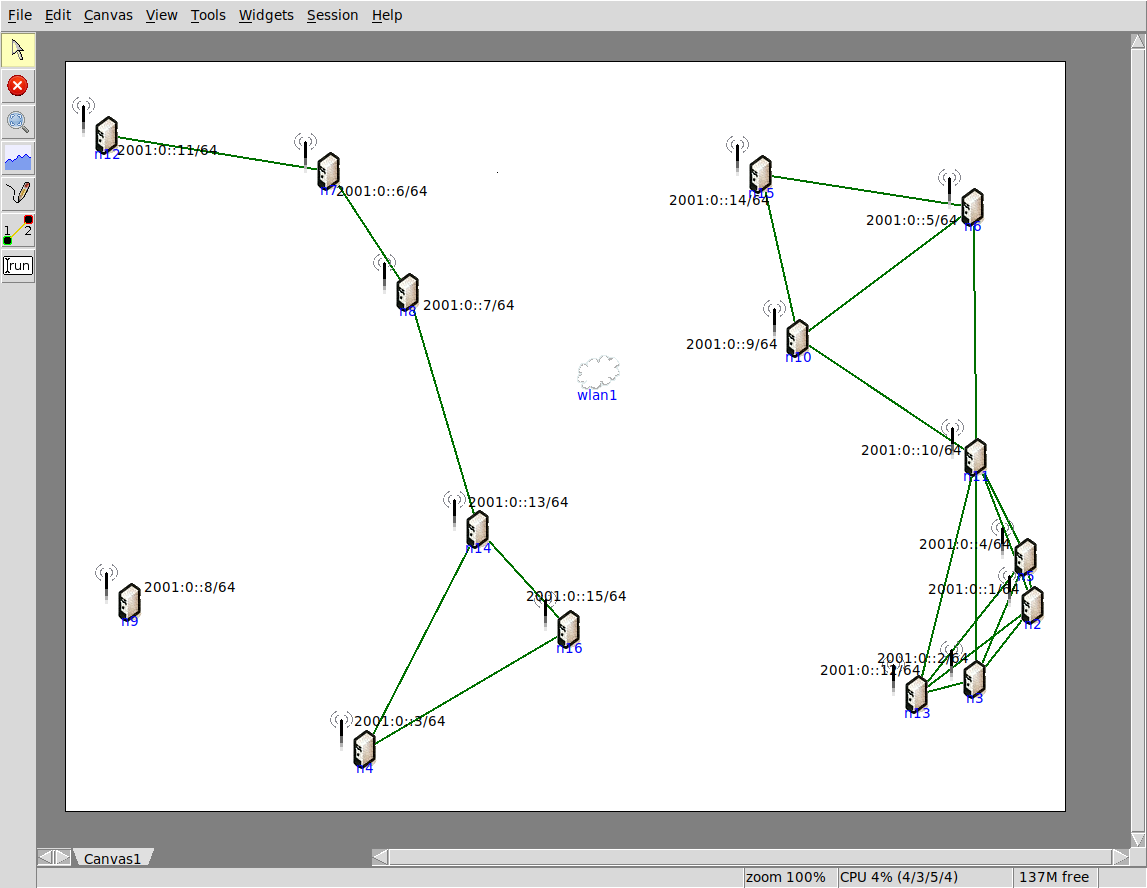
\includegraphics[width=0.6\linewidth,keepaspectratio]{include/core-screenshot}
  \end{figure}
\end{frame}

\begin{frame}
  \frametitle{Evaluation}

  \begin{itemize}
  \item Payload Size
  \begin{itemize}
    \item 64 KiB: compressed image
    \item 1 MiB: small image / short audio recording
    \item 5 MiB: smartphone image / audio recording
    \item 25 MiB: longer audio recording / short video
    \item 50 MiB: HD video
    \item 100 MiB: 4K smartphone video
  \end{itemize}
  \onslide<2>{
  \item{\acs{DTN} Software}
  \begin{itemize}
    \item DTN7
    \item Forban
    \item IBR-DTN
    \item Serval
  \end{itemize}
  }
  \end{itemize}
\end{frame}

\begin{frame}
  \frametitle{Two nodes}

  \begin{figure}
    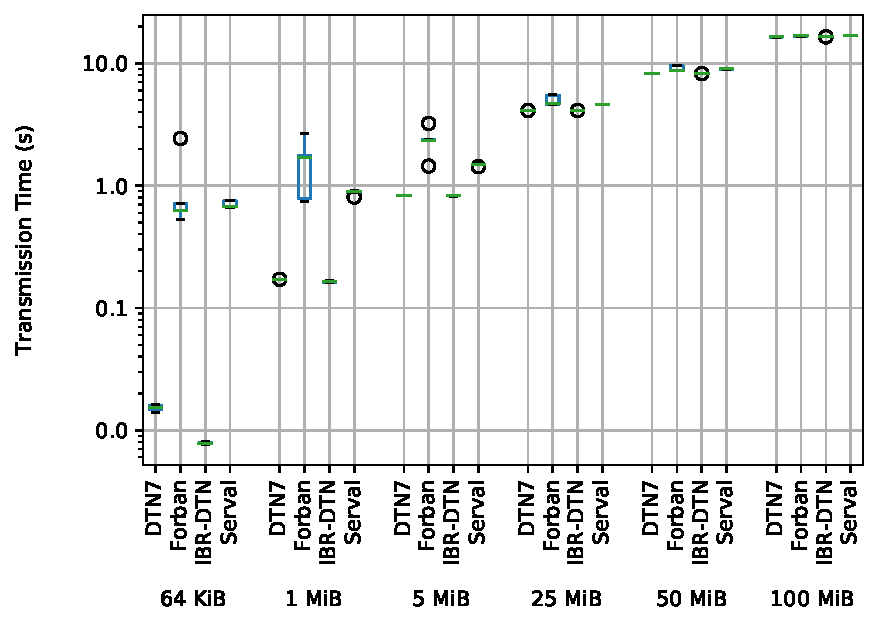
\includegraphics[width=\linewidth,keepaspectratio]{include/chain-runtimes-2}
  \end{figure}
\end{frame}

\begin{frame}
  \frametitle{64 nodes}

  \begin{figure}
    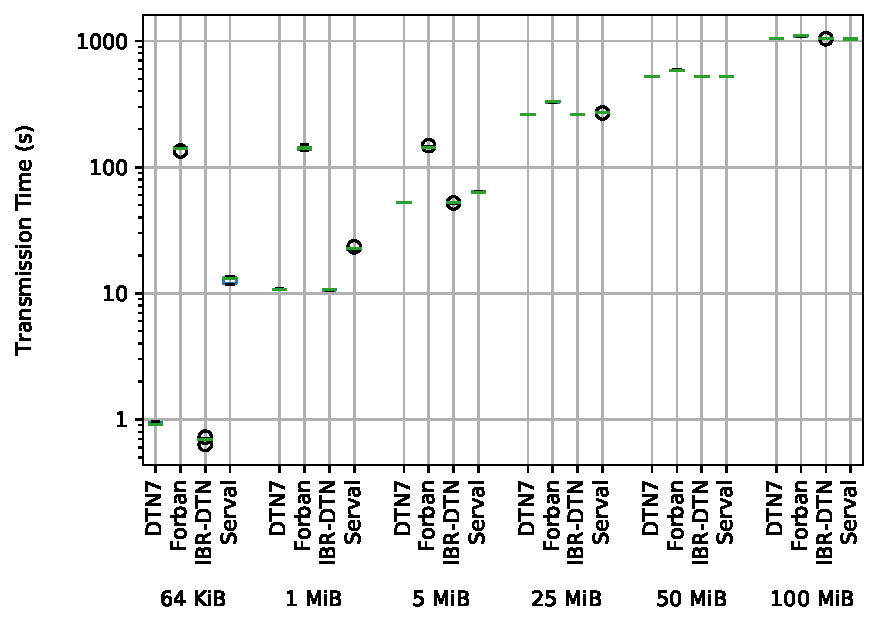
\includegraphics[width=\linewidth,keepaspectratio]{include/chain-runtimes-64}
  \end{figure}
\end{frame}
